% Это основная команда, с которой начинается любой \LaTeX-файл. Она отвечает за тип документа, с которым связаны основные правила оформления текста.
\documentclass{article}

% Здесь идет преамбула документа, тут пишутся команды, которые настраивают LaTeX окружение, подключаете внешние пакеты, определяете свои команды и окружения. В данном случае я это делаю в отдельных файлах, а тут подключаю эти файлы.

% Здесь я подключаю разные стилевые пакеты. Например возможности набирать особые символы или возможность компилировать русский текст. Подробное описание внутри.
\usepackage{packages}

% Здесь я определяю разные окружения, например, теоремы, определения, замечания и так далее. У этих окружений разные стили оформления, кроме того, эти окружения могут быть нумерованными или нет. Все подробно объяснено внутри.
\usepackage{environments}

% Здесь я определяю разные команды, которых нет в LaTeX, но мне нужны, например, команда \tr для обозначения следа матрицы. Или я переопределяю LaTeX команды, которые работают не так, как мне хотелось бы. Типичный пример мнимая и вещественная часть комплексного числа \Im, \Re. В оригинале они выглядят не так, как мы привыкли. Кроме того, \Im еще используется и для обозначения образа линейного отображения. Подробнее описано внутри.
\usepackage{commands}

% Пакет для титульника исследовательского проекта
\usepackage{titlepage}

% Пакет для кода
\usepackage{code}

% Ещё один уровень глав
%\setcounter{tocdepth}{4}
%\setcounter{secnumdepth}{4}

% Здесь задаем параметры титульной страницы
\setUDK{}
% Выбрать одно из двух
%\setToResearch
\setToProgram

\setTitle{3D renderer с нуля}
% \setStage{(промежуточный, этап 3)}
\setGroup{193}
%сюда можно воткнуть картинку подписи
\setStudentSgn{}
\setStudent{И.Н.Притуляк}
\setStudentDate{02.06.2021}
\setAdvisor{Дмитрий Витальевич Трушин}
\setAdvisorTitle{доцент, к.ф.-м.н.}
\setAdvisorAffiliation{ФКН НИУ ВШЭ}
\setAdvisorDate{}
\setGrade{}
%сюда можно воткнуть картинку подписи
\setAdvisorSgn{}
\setYear{2021}


% С этого момента начинается текст документа
\begin{document}

% Эта команда создает титульную страницу
\makeTitlePage

% Здесь будет автоматически генерироваться содержание документа
{
  \hypersetup{hidelinks}
  \tableofcontents
}

\newpage

% Данное окружение оформляет аннотацию: краткое описание текста выделенным абзацем после заголовка
\begin{abstract}
	Цель данной работы --- реализовать 3D-renderer с открытым исходным кодом.
	Реализация будет происходить с нуля, без использования низкоуровневых библиотек.
	Одной из основных целей также является изучить, как процесс рендеринга происходит снизу.
\end{abstract}

\section{Введение}

В приложениях, использующих 3D графику, часто стоит задача отображения объектов из виртуального 3D мира на 2D экран.
Процесс преобразования трёхмерной модели в двумерную картинку, которая впоследствии отображается на экране монитора, называется 3D-рендерингом.
Целью данного проекта является полностью с нуля реализовать программу, которая могла бы решать эту задачу.

В процессе реализации стоит несколько задач:

\begin{enumerate}
	\item Изучение принципов работы 3D-рендерера посредством изучения литературы, посвящённой данной теме.
	\item Краткое изложение необходимой теории.
	\item Написание на языке C++ библиотеки, позволяющей проецировать сцену на экран монитора, и приложения, демонстрирующего её работу.
	\item Описание архитектуры и дизайна реализации.
	\item Тестирование написанного кода и приведение его результатов.
	\item Написание сопроводительной документации, которая включает в себя инструкцию по работе с библиотекой и описание основных методов.
\end{enumerate}

Работа состоит из нескольких частей.
В первой части я рассказываю теорию, которая потребуется для реализации библиотеки, а также привожу алгоритмы, которые в ней используются.
Дальше идёт архитектура библиотеки.
Я рассказываю о том, какие классы она содержит и как эти классы взаимодействуют между собой.
Также в этой главе более подробно задевается алгоритм работы с библиотекой.
В следующей главе я поверхностно рассказываю реализацию основных методов, оцениваю их сложность.
В этой же главе обсуждается работа с таймером, подсчёт FPS и отрисовка каркаса.
В пятой главе прилагается инструкция по работе с библиотекой: что нужно настроить, и какие методы за это отвечают.
В заключение работы я привожу результаты тестирования на двух сценах с разными параметрами --- какой FPS вырабатывает рендерер и почему так происходит.

Большинство теоретического материала взято из книг~\cite{Graph3D} и~\cite{Math3d}, а также из интернета, а именно: процесс рендеринга~\cite[Chapter~1]{Math3d}, однородные координаты~\cite[Chapter~4.4]{Math3d}, барицентрические координаты~\cite[Chapter~IV.1.3]{Graph3D}, пирамида зрения~\cite[Chapter~5.3]{Math3d}, перемещение и вращение объектов~\cite[Chapter~4.3]{Math3d}, видовое преобразование~\cite{Camera}, перспективное преобразование~\cite[Chapter~5.5.1]{Math3d}, растеризация~\cite[Chapter~II.4]{Graph3D}.
Более подробно об этих вещах можно почитать по соответствующим сноскам.
Часть картинок также взяты из этих источников.

Репозиторий проекта располагается по следующей ссылке: \url{https://github.com/stabmind/3D-renderer}.

\subsection{Функциональные требования}

Библиотека должна предоставлять пользователю следующие возможности:

\begin{itemize}
	\item Отрисовка триангулированной 3D модели на экране монитора.
	\item Создание треугольника, который определяется тремя вершинами, заданными в любом порядке.
	Каждой вершине также соответствует какой-то цвет.
	\item Добавление треугольника или множества треугольников в мир.
	\item Задание параметров камеры, а также характеристик пирамиды зрения.
	\item Задание параметров окна, в котором будет отображаться проекция.
	\item Возможность повернуть камеру на любой угол относительно любого вектора, в том числе каждой оси.
	\item Возможность запустить интерактивный режим, в котором при помощи клавиатуры можно вращать и перемещать камеру, тем самым перемещаясь по миру.
	\item Возможность запустить динамический режим, в котором камера вращается по окружности вокруг центра.
	\item Возможность включить отображение количества кадров в секунду, которые генерирует рендерер.
	\item Возможность включить отрисовку каркаса, цвет которого также можно настроить.
\end{itemize}

Более подробное объяснение того, какие конкретно параметры нужно настроить и каковы функции описанных объектов, будет объяснено далее.

\subsection{Нефункциональные требования}

\begin{enumerate}
	\item Требования к надёжности.
	Если метод требует некоторый формат входных данных, например неотрицательные значения параметров окна, и пользовательские данные ему не соответствуют, то программа возвращает соответствующее исключение.
	\item Требования к программному обеспечению.
	\begin{itemize}
		\item Язык программирования: C++ с поддержкой стандарта C++20.
		\item Компилятор: g++ 10.3.1.
		\item Используемые библиотеки: SFML \footnote{\url{https://www.sfml-dev.org}} и Eigen \footnote{\url{https://eigen.tuxfamily.org}} --- для взаимодействия с пользователем (ввод с клавиатуры, вывод готового изображения на экран монитора) и работы с матрицами соответственно.
		Из первой библиотеки также используется таймер: для подсчёта FPS и при реализации движения камеры.
		\item Система контроля версий: Git.
		\item Система сборки: CMake версии 3.7.2 или более новой.
	\end{itemize}
	\item Требования к оформлению кода.
	\begin{itemize}
		\item Style guide: Google \footnote{\url{https://google.github.io/styleguide/cppguide.html}}.
		\item Программа по форматированию в соответствии со style guide: Clang.
	\end{itemize}
	\item Системные требования.
	Для использования библиотеки достаточно, чтобы операционная система нормально функционировала.
\end{enumerate}

\newpage

\section{Теория}

Прежде чем разобраться с архитектурой библиотеки, кратко изучим теорию, которая за ней лежит.
Весь процесс делится на два этапа: настройка рендерера и обработка рендерером поставленной сцены, результатом которой будет изображение на экране монитора.
Настройка рендерера будет рассмотрена в главе \ref{instruction section}, она подразумевает постановку сцены, то есть задание триангулированной модели посредством такого примитива как треугольник, и задание камеры, при помощи которой будет происходить рендеринг модели на экран монитора.
Сам рендеринг происходит в несколько этапов: модельное преобразование, видовое преобразование, клиппинг (\emph{clipping}), перспективное преобразование и растеризация (рис. \ref{pipeline}).
В основе рендеринга лежит \emph{z-буферизация} --- способ отрисовки изображения в зависимости от расстояния до экрана, за которое отвечает $z$ координата.

На протяжении всей работы нам потребуются следующие системы координат:

\begin{enumerate}
	\item Локальная система координат --- система координат, индивидуальная для каждого объекта
	\item Глобальная система координат --- система координат, в которой располагается сцена.
	\item Система координат относительно камеры --- система координат, в которой происходит перспективное преобразование.
	\item Homogeneous clip space --- система координат, которая получается перспективным преобразованием.
\end{enumerate}

Все преобразования между этими системами координат происходят в пространстве $\R^{4}$ при помощи однородных координат посредством следующих матриц:

\begin{enumerate}
	\item Model matrix --- преобразование из локальной системы координат в глобальную.
	\item View matrix --- преобразование из глобальной системы координат в систему координат относительно камеры.
	\item Projection matrix --- преобразование из системы координат относительно камеры в homogeneous clip space.
\end{enumerate}

Переходы между системами координат идут в описанном выше порядке.
Однако прежде чем произвести перспективное преобразование происходит клиппинг --- процедура, когда удаляется часть модели, которая не попадает на экран.
После перспективного преобразования мы оказываемся в Homogeneous clip space, в этом пространстве все точки имеют нормализованные координаты, теперь их удобно проецировать на экран.
Итоговые треугольники проходят процесс растеризации, а затем готовое изображение отображается на экране монитора.

\begin{figure}[ht]
    \center{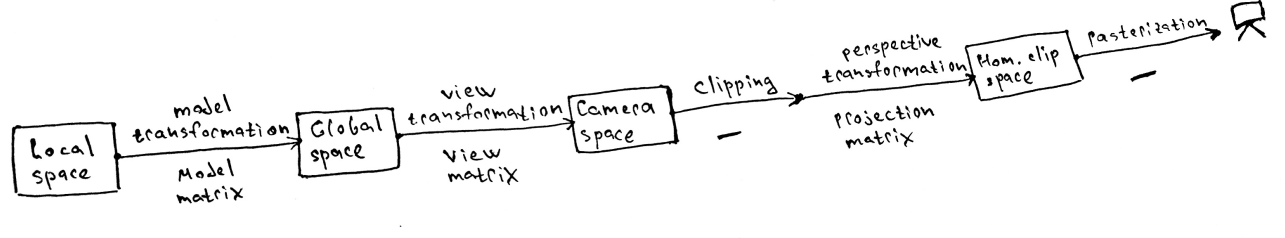
\includegraphics[scale=0.35]{images/pipeline.png}}
    \caption{Pipeline. Там, где происходят преобразования из одной системы координат в другую, сверху подписано преобразование, а снизу --- матрица при помощи которой оно происходит.}
    \label{pipeline}
\end{figure}

\subsection{Основные понятия}

\subsubsection{Однородные координаты}

Перед рассмотрением процесса рендеринга удобно сначала обсудить, что такое однородные координаты и зачем они нужны.
Однородные координаты удобны тем, что позволяют произвести поворот и смещение точки относительно какого-то вектора одним только домножением на соответствующую матрицу.
При этом, если мы рассматриваем не точку, а вектор, то для него то же домножение будет давать только лишь поворот.
Однородные координаты также удобны при перспективном преобразовании, обсуждение которого идёт дальше.

В $\R^{3}$ мы различаем точки и векторы, поэтому сопоставим им соответствующие однородные координаты:
\begin{enumerate}
	\item
	Пусть $P = (P_{x}, P_{y}, P_{z})$ --- точка в $\R^{3}$.
	Тогда $\widetilde{P} = (P_{x}, P_{y}, P_{z}, 1)$ --- её однородные координаты в $\R^{4}$.
	\item
	Пусть $\vec{V} = (V_{x}, V_{y}, V_{z})$ --- вектор в $\R^{3}$.
	Тогда $\widetilde{V} = (V_{x}, V_{y},V_{z} , 0)$ --- его однородные координаты в $\R^{4}$.
\end{enumerate}

В $\R^{4}$ мы различаем только вектора.
Пусть $\widetilde{C} = (C_{x}, C_{y}, C_{z}, w)$ --- вектор в $\R^{4}$.
Если $w$ равняется нулю, то $\widetilde{C}$ соответствует вектор в $\R^{3}$ равный $\vec{V} = (C_{x}, C_{y}, C_{z})$.
В противном случае ему соответствует точка равная $P = (\frac{C_{x}}{w}, \frac{C_{y}}{w}, \frac{C_{z}}{w})$.
Отсюда также следует, что векторам $\widetilde{C}$ и $\lambda \widetilde{C}$ соответствует одна точка в $\R^{3}$, если только $\lambda$ и $w$ не равны нулю.

\subsubsection{Барицентрические координаты}

На этапе удаления частей треугольника, которые не попадают на экран, потребуются барицентрические координаты.
Пусть $x$, $y$ и $z$ неколлинеарные вершины треугольника.
Пусть также вершина $u$ лежит внутри или на границе треугольника.
Тогда её можно представить единственным образом в виде $u = \alpha x + \beta y + \gamma z$, где $\alpha + \beta + \gamma = 1$, и $(\alpha, \beta, \gamma)$ --- её барицентрические координаты.

Пусть вершина $u$ разбивает треугольник на три области: $A$, $B$ и $C$ (рис. \ref{barycent}).
Тогда можно посчитать её барицентрические координаты следующим образом:

\begin{gather*}
	\alpha = \frac{A}{A + B + C} \\
	\beta = \frac{B}{A + B + C} \\
	\gamma = \frac{C}{A + B + C}
\end{gather*}

\begin{figure}[ht]
    \center{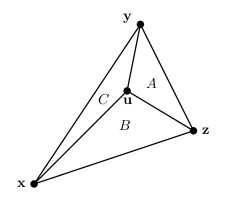
\includegraphics[scale=0.5]{images/barycent.png}}
    \caption{Разбиение треугольника для вычисления барицентрических координат вершины $u$.}
    \label{barycent}
\end{figure}

Зная барицентрические координаты, можно интерполировать функцию $f$ на вершину $u$:

\begin{equation*}
	f(u) = \alpha f(x) + \beta f(y) + \gamma f(z)
\end{equation*}

\subsubsection{Пирамида зрения} \label{view frustum section}

Обсудим, что представляет из себя камера и что такое пирамида зрения.
В локальной системе координат камера представляет из себя точку в начале отсчёта и имеет направление, задаваемое некоторым вектором.
На расстоянии $n$ от этой точки вдоль направляющего вектора в перпендикулярной ему плоскости располагается прямоугольный экран, на который впоследствии будет производиться проекция модели.
Параллельно экрану на б\'{о}льшем расстоянии $f$ аналогично проходит ещё одна плоскость.
Вместе с тем из центра координатной оси через стороны экрана область ограничивают ещё четыре плоскости.
Часть модели, которая попала в эту область, будет проецироваться на экран.
Конструкция же называется \emph{пирамидой зрения} (рис. \ref{view frustum}).

\begin{figure}[ht]
    \center{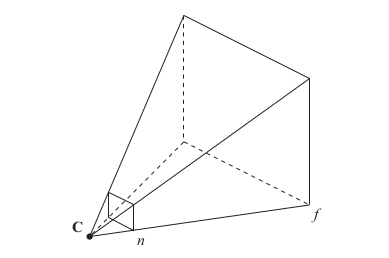
\includegraphics[scale=0.5]{images/view frustum.png}}
    \caption{Пирамида зрения.}
    \label{view frustum}
\end{figure}

\subsection{Перемещение и вращение объектов}

Чтобы понять как перемещать и вращать объекты, достаточно научиться делать то же самое для точек.
Как сместить точку на некоторый вектор очевидно --- нужно просто прибавить к точке требуемый вектор смещения.
С вращением же всё немного сложнее.
Мы хотим повернуть точку $v$ на угол $\theta$ относительно единичного вектора $\vec{u}$ по часовой стрелке (рис. \ref{rotation}).
Для этого достаточно сделать домножение на матрицу $R_{u}(\theta)$ следующего вида:

\begin{equation*}
	R_{u}(\theta) =
		\begin{pmatrix}
			\cos{\theta} + (1 - \cos{\theta})u_{x}^{2} & (1 - \cos{\theta})u_{x}u_{y} - \sin{\theta} u_{z} & (1 - \cos{\theta})u_{x}u_{z} + \sin{\theta} u_{y} \\
			(1 - \cos{\theta})u_{x}u_{y} + \sin{\theta} u_{z} & \cos{\theta} + (1 - \cos{\theta})u_{y}^{2} & (1 - \cos{\theta})u_{y}u_{z} - \sin{\theta} u_{x} \\
			(1 - \cos{\theta})u_{x}u_{z} - \sin{\theta} u_{y} & (1 - \cos{\theta})u_{y}u_{z} + \sin{\theta} u_{x} & \cos{\theta} + (1 - \cos{\theta})u_{z}^{2}
		\end{pmatrix}
\end{equation*}

\begin{figure}[ht]
	\center{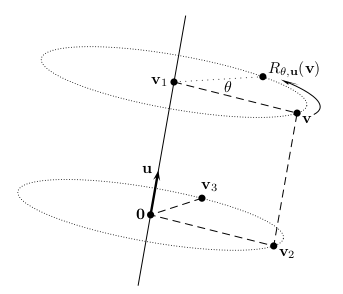
\includegraphics[scale=0.5]{images/rotation.png}}
	\caption{Поворот точки $v$ относительно единичного вектора $\vec{u}$ на угол $\theta$ по часовой стрелке.}
	\label{rotation}
\end{figure}

\subsection{Модельное преобразование}

Чтобы перевести объект из локальной системы координат в глобальную, используется модельное преобразование.
И хотя непосредственно в реализации оно не используется, его полезно рассмотреть для полноты изложения.
Объекты хранятся в локальной системе координат и при помощи модельной матрицы каждый объект переходит в глобальную систему координат.
Данное преобразование происходит при помощи смещения объекта на некоторый вектор.
Если $\vec{h} = (h_{x}, h_{y}, h_{z})$ --- вектор смещения, то матрица преобразования $M_{\text{model}}$ примет следующий вид:

\begin{equation*}
	M_{\text{model}} =
		\begin{pmatrix}
			1 & 0 & 0 & h_{x} \\
			0 & 1 & 0 & h_{y} \\
			0 & 0 & 1 & h_{z} \\
			0 & 0 & 0 & 1
		\end{pmatrix}
\end{equation*}

\subsection{Видовое преобразование} \label{view transform section}

Когда мы научились переводить объекты из локальной системы координат в глобальную, следующим преобразованием будет видовое.
Данное преобразование переводит объекты из глобальной системы координат в систему координат относительно камеры.
Пусть камера имеет направление $\vec{v}_{c}$, и задан некоторый неколлинеарный вектор $\vec{u}$.
При помощи этих двух векторов зададим новую систему координат, базисы которой образуют левую тройку: ось $z$ направлена противоположно $\vec{v}_{c}$, ось $x$ смотрит вправо, а $y$ --- вверх.
Пусть векторы $e'_{1}$, $e'_{2}$ и $e'_{3}$ задают новые оси $x$, $y$ и $z$ соответственно.
Тогда пример такой системы будет изображён на рисунке \ref{camera axes}.

\begin{figure}[ht]
    \center{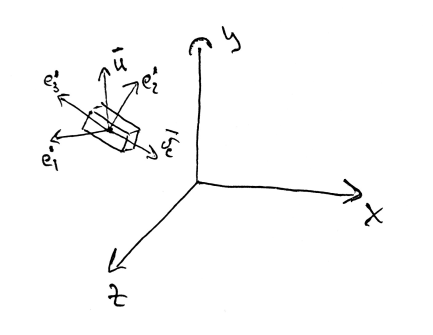
\includegraphics[scale=0.5]{images/camera axes.png}}
    \caption{Пример новой системы координат относительно камеры. \\ Векторы $e'_{1}$, $e'_{2}$ и $e'_{3}$ задают новые оси $x$, $y$ и $z$ соответственно.}
    \label{camera axes}
\end{figure}

Новый базис будет иметь следующий вид:

\begin{gather*}
	e'_{1} = \frac{\vec{v}_{c} \times \vec{u}}{||\vec{v}_{c} \times \vec{u}||} \\
	e'_{2} = -\frac{\vec{v}_{c} \times e'_1}{||\vec{v}_{c} \times e'_1||} \\
	e'_{3} = -\frac{\vec{v}_{c}}{||\vec{v}_{c}||}
\end{gather*}

Пусть $\vec{h}$ --- смещение камеры.
По построению матрица $C = (e'_{1}, e'_{2}, e'_{3})$ --- ортогональная матрица перехода из стандартного базиса в новый.
Тогда матрица видового преобразования $M_{\text{view}}$ имеет вид

\begin{equation*}
	M_{\text{view}} =
		\left(
			\begin{array}{c|c}
				\mbox{\Large $C^{T}$} &
				\begin{array}{c}
					0 \\ 0 \\ 0
				\end{array} \\ \hline
				\begin{array}{ccc}
					0 & 0 & 0
				\end{array} & 1
			\end{array}
		\right)
		\cdot
		\left(
			\begin{array}{c|c}
				\mbox{\Large $E$} &
				\begin{array}{c}
					\\ \mbox{\Large $-\vec{h}$} \\ \\
				\end{array} \\
				\hline
				\begin{array}{ccc}
					0 & 0 & 0
				\end{array} & 1
			\end{array}
		\right)
\end{equation*}

\subsection{Клиппинг}

Прежде чем произвести перспективное преобразование, удалим части треугольника, которые не попадают на экран.
Урезать треугольник будем сначала в координатах $x$ и $z$, а затем в координатах $y$ и $z$.
В каждом случае стоит задача клиппинга двумерного треугольника трапецией.
Для удобства, не умаляя общности, переименуем координаты и будем считать, что мы находимся в координатах $x$ и $y$.
Тогда применим следующий алгоритм:

\begin{enumerate}
	\item Сначала сохраним вершины треугольника, которые лежат внутри трапеции, их $z$ координата нам уже известна.
	\item Затем сохраним вершины трапеции, которые лежат внутри треугольника.
	Чтобы интерполировать их $z$ координату, посчитаем при помощи векторного произведения площади, необходимые для вычисления барицентрических координат.
	\item Теперь попарно пересечём стороны треугольника и стороны трапеции.
	Точки пересечения также интерполируем, но в этот раз считая лишь отношение длин, и сохраним их.
	\item В конце, когда у нас есть вершины, которые задают выпуклый многоугольник, мы его триангулируем.
	Для этого зафиксируем самую левую нижнюю вершину $v$, отсортируем относительно неё по полярному углу остальные.
	Затем проведём рёбра между вершиной $v$ и всеми остальными, а также между соседними вершинами.
\end{enumerate}

Может быть такое, что полученный для триангуляции многоугольник лежит в перпендикулярной для нас плоскости.
В этом случае перед триангуляцией нужно найти пару координат, в которой это условие нарушается и далее работать в ней.

В приведённом выше алгоритме возникает подзадача проверки принадлежности вершины $u$ некоторому многоугольнику.
Она решается следующим образом:

\begin{enumerate}
	\item Переберём все тройки смежных вершин многоугольника.
	\item Для каждой конкретной тройки сопоставим названия $a$, $b$ и $c$, где вершина $b$ находится посередине.
	\item Тогда в каждом случае должно выполняться условие, что $\langle b - a, c - a \rangle$ и $\langle b - a, u - a \rangle$ не имеют противоположные знаки, то есть лежат по одну сторону от ребра $(a, b)$, включая само ребро.
\end{enumerate}

Пример возможного результата клиппинга изображён на рисунке \ref{clipping}.

\begin{figure}[ht]
    \center{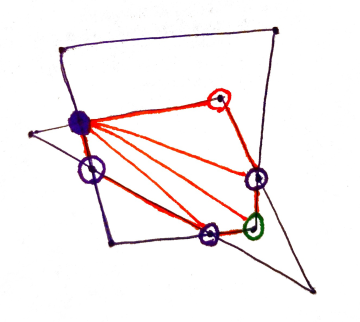
\includegraphics[scale=0.5]{images/clipping.png}}
    \caption{Возможный результат клиппинга. \\
    		 Красные вершины добавляются на первом этапе, зелёные --- на втором, фиолетовые --- на третьем. \\
    		 На четвёртом этапе происходит триангуляция: выбирается фиолетовая закрашенная вершина и проводятся оранжевые рёбра.}
    \label{clipping}
\end{figure}

\subsection{Перспективное преобразование}

Предпоследним этапом в процессе построения двумерной картинки является перспективное преобразование.
Чтобы понять, как оно работает, рассмотрим систему координат, полученную на предыдущем этапе.
Пусть левый нижний угол экрана имеет координаты $(l, b, -n)$, правый верхний --- $(r, t, -n)$ (рис. \ref{camera space}).

\begin{figure}[ht]
    \center{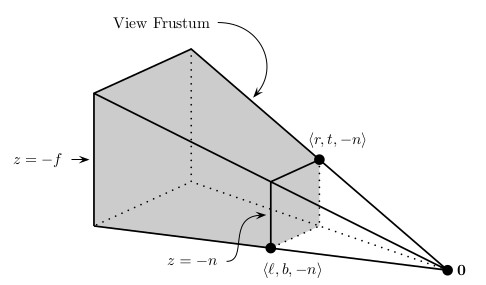
\includegraphics[scale=0.5]{images/camera space.png}}
    \caption{Пространство камеры.}
    \label{camera space}
\end{figure}

Суть перспективного преобразования заключается в том, что мы преобразуем область, ограниченную пирамидой зрения, в квадрат $2 \times 2 \times 2$ с центром в начале координат (рис. \ref{perspective projection}).
Полученные координаты интерпретируются следующим образом: $x$ и $y$ задают нормированное положение на экране, а $z$ является глубиной, которая потом используется для отрисовки пикселей на растровом экране.

\begin{figure}[ht]
    \center{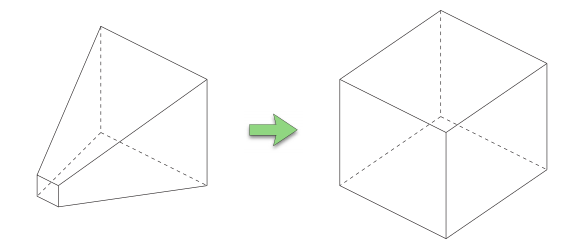
\includegraphics[scale=0.5]{images/perspective projection.png}}
    \caption{Перспективное преобразование.}
    \label{perspective projection}
\end{figure}

Матрицей перспективного преобразования является матрица $M_{\text{proj}}$, которая имеет следующий вид:

\begin{equation*}
	M_{\text{proj}} =
		\begin{pmatrix}
			\dfrac{2n}{r - l}	& 0					& \dfrac{r + l}{r - l}	& 0 \\
			0					& \dfrac{2n}{t - b}	& \dfrac{t + b}{t - b}	& 0 \\
			0					& 0					& -\dfrac{f + n}{f - n}	& -\dfrac{2nf}{f - n} \\
			0					& 0					& -1					& 0
		\end{pmatrix}
\end{equation*}

Отмечу одно из важных свойств, которое даёт перспективное преобразование, оно потребуется при интерполяции глубины треугольника --- координата $z$ теперь может быть интерполирована линейно, выражая при этом корректное расстояние от экрана монитора.

\subsection{Растеризация} \label{rasterization section}

Последним этапом рендеринга является растеризация.
Во время растеризации происходит переход из нормированной системы координат в окончательную картинку, которая затем будет изображена на экране.
Но прежде чем растеризовать изображение, получим его координаты на экране монитора.
Пусть экран имеет ширину $w$ и высоту $h$.
Пусть также точка $p = (x, y, z)$ принадлежит кубу, соответствующему нормированной системе координат.
Тогда, применив линейное преобразование, получаем новые координаты следующим образом:

\begin{equation*}
	x' = \frac{x + 1}{2} w \quad \text{и} \quad y' = \frac{y + 1}{2} h
\end{equation*}

Округляя новые координаты вниз, получаем растровые координаты $(i, j)$ такие, что $0 \le i < w$, $0 \le j < h$:

\begin{equation*}
	i = \min(\floor{x'}, w - 1) \quad \text{и} \quad j = \min(\floor{y'}, h - 1)
\end{equation*}

Теперь мы хотим научиться отрисовывать треугольники.

\subsubsection{Отрисовка отрезка}

Прежде чем отрисовывать весь треугольник, научимся отрисовывать отрезки.
Пусть мы хотим провести отрезок между двумя точками с растровыми координатами $(i_{1}, j_{1})$ и $(i_{2}, j_{2})$.
Не умаляя общности, мы считаем что $i_{1} < i_{2}$.
В силу симметрии можно считать что $j_{1} < j_{2}$.
Пусть также $\Delta i = i_{2} - i_{1}$ и $\Delta j = j_{2} - j_{1}$.
Снова в силу симметрии считаем что $\frac{\Delta j}{\Delta i} \le 1$.
Откуда вытекает следующий факт: для каждого $i$ такого что $i_{1} \le i \le i_{2}$ существует только один закрашенный пиксель с координатами $(i, j)$ для некоторого $j$ (отрезок $AB$ на рис. \ref{rasterized line}).

\begin{figure}[ht]
    \center{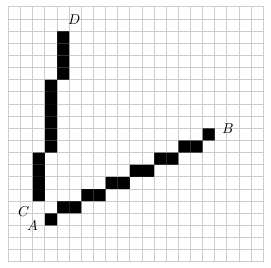
\includegraphics[scale=0.5]{images/rasterized line.png}}
    \caption{Пример отрисовки прямых на растровом экране.}
    \label{rasterized line}
\end{figure}

Пусть $\alpha = \frac{i - i_{1}}{i_{2} - i_{1}}$ и $j(i) = [(1 - \alpha) j_{1} + \alpha j_{2}]$.
Тогда пиксели $(i, j(i))$, закрашенные для каждого $i$ от $i_{1}$ до $i_{2}$, образуют требуемую прямую на растровом экране.
Аналогичным образом делается интерполяция глубины, то есть $z(i) = [(1 - \alpha)z_{1} + \alpha z_{2}]$.

Итого получаем следующий алгоритм:

\begin{enumerate}
	\item Проверяем условие $\left| \frac{\Delta j}{\Delta i} \right| \le 1$.
	Если оно не выполняется, то меняем координаты $x$ и $y$ местами, отмечаем этот факт каким-нибудь флагом.
	\item Проверяем условие $i_{1} < i_{2}$.
	Если оно не выполняется, то меняем точки местами.
	\item В цикле от $i_{1}$ до $i_{2}$ вычисляем $j(i)$ и $z(i)$ по формулам выше.
	Тем самым, учитывая состояние флага, мы получаем требуемые координаты и глубину пикселя на растровом экране.
\end{enumerate}

\subsubsection{Отрисовка треугольника}

Теперь мы готовы отрисовать треугольник.
Идея следующая: сначала отрисуем его стороны, а затем будем просто идти снизу вверх внутри ограничивающего его прямоугольника и отрисовывать точно таким же образом отрезки, концами которых будут точки пересечения соответствующих горизонтальных прямых с треугольником (рис. \ref{triangle rasterization}).

\begin{figure}[ht]
    \center{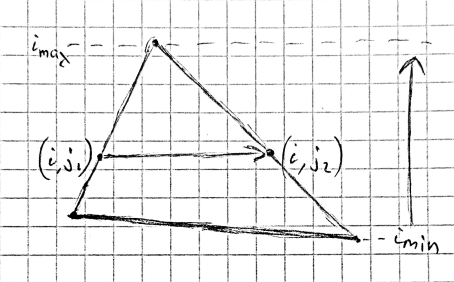
\includegraphics[scale=0.5]{images/triangle rasterization.png}}
    \caption{Итерация отрисовки треугольника.}
    \label{triangle rasterization}
\end{figure}

Для того, чтобы построить точный алгоритм, сначала определим границы цикла, отвечающего за проход строк, где идёт пересечение и отрисовка, а затем научимся определять сами точки пересечения.
Пусть $i_{1}$, $i_{2}$ и $i_{3}$ --- $i$ координаты соответствующих вершин.
Тогда границами внешнего цикла будут

\begin{equation*}
	i_{\text{min}} = \min(i_{1}, i_{2}, i_{3}) \quad \text{и} \quad i_{\text{max}} = \max(i_{1}, i_{2}, i_{3})
\end{equation*}

Чтобы определить пересечение, во время отрисовки сторон запомним для каждого $i$ точки с минимальным и максимальным $j$ --- они будут концами отрезка, который затем нужно отрисовать.

Итого получаем следующий алгоритм:

\begin{enumerate}
	\item Отрисовываем стороны треугольника, попутно запоминая для каждой строки точки с минимальной и максимальной координатой $j$.
	\item Идём по строкам от $i_{\text{min}}$ до $i_{\text{max}}$ и отрисовываем соответствующие им отрезки.
\end{enumerate}

\newpage

\section{Архитектура} \label{architecture section}

После того как мы разобрались с теорией, рассмотрим архитектуру библиотеки --- из каких классов она состоит и как эти классы взаимодействуют между собой.
Библиотека содержит следующие классы:

\begin{enumerate}
	\item \verb"Triangle".
	Для обработки сцены рендерер требует, чтобы модель была триангулирована, поэтому каждая модель обязана быть представлена как композиция треугольников.
	Данный класс отвечает за то, чтобы представлять эти треугольники.
	Он предоставляет методы установки вершин и их цветов, получения вершин и их цветов, получения итераторов для обхода всех вершин.
	\item \verb"World".
	Все треугольники хранятся в единой системе координат, называемой миром.
	Данный класс является их хранилищем.
	Он предоставляет методы добавления одного треугольника или нескольких треугольников сразу, а также методы получения итераторов для обхода всех треугольников в мире.
	\item \verb"Camera".
	Каждый треугольник проецируется на экран при помощи камеры.
	Данный класс нужен, чтобы задать параметры камеры и соответствующей ей пирамиды зрения, которые нужны для составления матриц видового и перспективного преобразований.
	Он предоставляет методы установки данных параметров, методы поворота и смещения камеры, методы получения матриц описанных преобразований, методы получения параметров пирамиды зрения.
	\item \verb"Screen".
	Проецирование модели происходит на экран монитора в отдельном окне.
	Данный класс используется, чтобы хранить готовое изображение, которое затем отображается на экране.
	Он предоставляет методы по установке размеров окна и параметров пикселей, получения размеров окна, цвета пикселя и его глубины, а также метод для очистки экрана.
	\item \verb"Renderer".
	По имеющимся классам \verb"World" и \verb"Camera", которые задают сцену, нужно получить итоговую картинку в классе \verb"Screen".
	Данный класс по заданным ему миру и камере производит проекцию модели, готовое изображение которой помещается в экран.
	Он имеет метод, который осуществляет процесс выше, а также методы активации режима отображения каркаса и установки его цвета.
	\item \verb"Application".
	Чтобы связать все вышеописанные классы вместе, используется класс \verb"Application".
	Он предоставляет методы настройки мира, камеры, экрана и рендерера, метод активации отображения FPS.
	Также имеются методы запуска интерактивного и динамического режима.
\end{enumerate}

Рассмотрим взаимодействие представленных классов.
Основным из них является класс \verb"Application", именно при помощи него происходит настройка всех компонентов, а затем запуск требуемого режима.
Этот класс содержит в себе классы \verb"World", \verb"Camera", \verb"Screen" и \verb"Renderer".
После их настройки вызывается один из методов: \verb"RunInteractiveScene" или \verb"RunRotatingScene".
Каждый из этих методов создает окно на экране монитора, в которое будет отображаться спроецированная модель, а затем запускает бесконечный цикл, который в первом случае при нажатии клавиш клавиатуры перемещает или поворачивает камеру, тем самым изменяя картинку в окне, а во втором --- самостоятельно вращает камеру, тем самым создавая анимацию без участия пользователя.
Для получения готового изображения на каждой итерации цикла вызывается метод \verb"Render" класса \verb"Renderer", который принимает на вход классы \verb"World", \verb"Camera" и \verb"Screen".
Результат его работы сохраняется в последнем из них.
Также отметим, что поскольку мир является хранилищем треугольников, то класс \verb"World" для своей реализации непосредственно использует класс \verb"Triangle".
На рисунке \ref{architecture} изображено визуальное представление описанного выше взаимодействия.

\begin{figure}[ht]
    \center{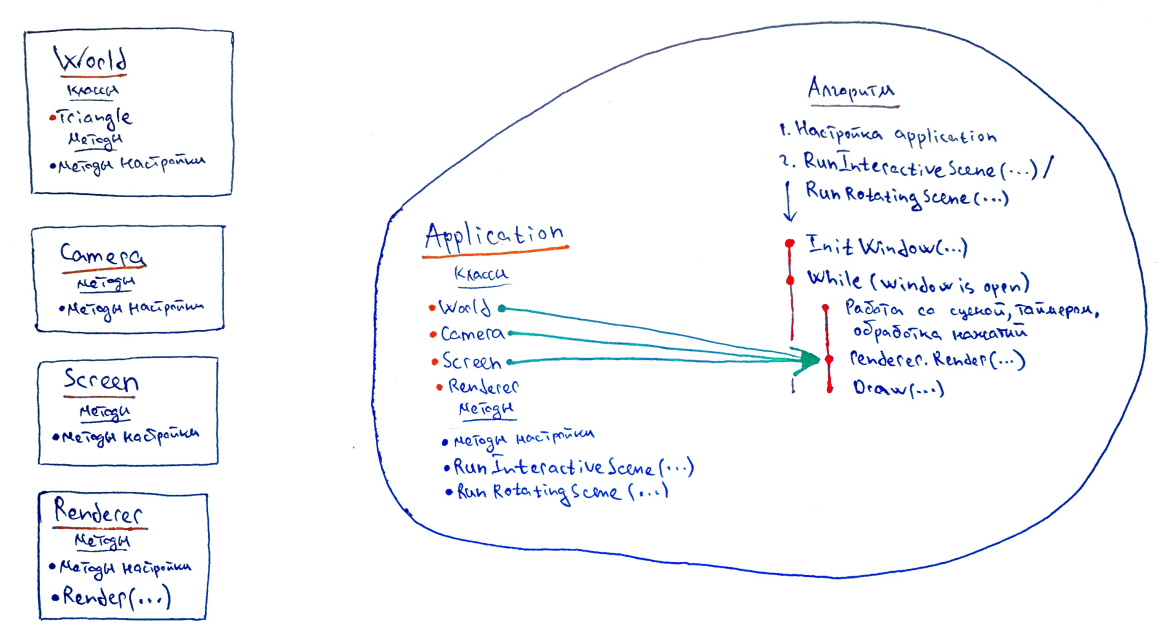
\includegraphics[scale=0.4]{images/architecture.png}}
    \caption{Архитектура проекта. Точки оранжевого цвета отмечают классы, которые в явном виде хранит основной класс, а точки фиолетового цвета --- методы, необходимые для функционирования всей системы.}
    \label{architecture}
\end{figure}

\newpage

\section{Детали реализации и сложность алгоритмов}

\subsection{Метод Render}

Алгоритм работы метода \verb"Render" класса \verb"Renderer" следующий:
\begin{enumerate}
	\item Подготавливаем рендерер и очищаем экран.
	Это занимает $O(w \cdot h)$ времени.
	\item Пробегаемся по треугольникам в мире, производим с каждым из них видовое преобразование, клиппинг, перспективное преобразование и растеризацию.
	В силу константности количества вершин у треугольника и трапеции данный процесс занимает $O(n \cdot w \cdot h)$ времени, где $n$ --- количество треугольников.
\end{enumerate}

Итого получаем затраты $O(n \cdot w \cdot h)$ времени и $O(n + w \cdot h)$ памяти.

\subsection{Методы RunInteractiveScene, RunRotatingScene и подсчёт FPS}

План работы методов \verb"RunInteractiveScene" и \verb"RunRotatingScene" описан в главе \ref{architecture section}.
Здесь я уточню часть, где происходит работа со сценой, таймером и обработкой нажатий.
В начале исполнения каждого из этих методов создаётся таймер, который замеряет время, уходящее на очередную итерацию цикла.
Пусть очередная итерация цикла отработала за $t$ секунд.
Если активирован режим отображения FPS, то поверх сгенерированного изображения отображается округлённое количество кадров в секунду равное $\frac{1}{t}$.
Если скорость движения камеры $v$, а скорость изменения угла $u$, то при необходимости движения или поворота, то есть при реакции на нажатие соответствующих клавиш, они будут произведены со скоростью $v \cdot t$ и $u \cdot t$ соответственно.
Это обеспечивает одинаковую скорость движения при работе на компьютерах разной мощности.

Отдельно рассмотрим движение камеры при выполнении метода \verb"RunRotatingScene".
На вход этот метод принимает длину радиуса $r$ и скорость вращения $v$.
Если поддерживать счётчик $s$, то на очередной итерации к нему прибавляется значение $v \cdot t$, а новые координаты камеры следующие: $x = r \sin(s)$, $y = r \cos(s)$, $z = 0$.

\subsection{Отрисовка каркаса}

В главе \ref{rasterization section} я описал, как происходит процесс растеризации.
Здесь я опишу, какие доработки вносятся, чтобы добавить отрисовку каркаса.
Для этого нам потребуется ещё один двумерный массив, в котором мы будет отмечать, принадлежит ли очередной пиксель ребру треугольника.
Теперь во время отрисовки рёбер вместо их настоящего цвета будем ставить цвет каркаса, но запоминать настоящие параметры пикселя, а также отмечать принадлежность пикселя ребру.
Во время же растеризации непосредственно треугольника остаётся лишь учитывать, является ли этот пиксель <<свободным>>.

\newpage

\section{Инструкция по работе с библиотекой} \label{instruction section}

В главе \ref{architecture section} описан процесс того, как работает библитека.
Этого почти достаточно, чтобы уже начать ею пользоваться.
Осталось понять как настраивать класс \verb"Application".
Чтобы его настроить, необходимо задать параметры мира, камеры, экрана, рендерера и самого application.
Делается это при помощи описанных ниже методов.

Методы для настройки мира:
\begin{itemize}
	\item \verb"void AddTriangle(const Triangle &triangle);" \\
	Добавляет треугольник в мир.
	\item \verb"void AddTriangles(const World::TriangleVec &triangles);" \\
	Добавляет вектор треугольников в мир.
\end{itemize}

Методы выше требуют треугольник.
Ниже приведён пример, в котором создаётся треугольник с вершинами $(1, 0, 0)$, $(0, 1, 0)$ и $(0, 0, 1)$.
Им назначаются красный, зелёный и синий цвета соответственно.

\begin{cppcode}
  Vertex v1({1, 0, 0}, {255, 0, 0});
  Vertex v2({0, 1, 0}, {0, 255, 0});
  Vertex v3({0, 0, 1}, {0, 0, 255});
  Triangle triangle(v1, v2, v3);
\end{cppcode}

Методы для настройки камеры:
\begin{itemize}
	\item \verb"void setCamera(double x1, double y1, double z1, double x2, double y2, double z2);" \\
	Задаёт координаты местоположения камеры $(x_{1}, y_{1}, z_{1})$ и её направление $(x_{2}, y_{2}, z_{2})$.
	\item \verb"void setCameraPosition(double x, double y, double z);" \\
	Задает местоположение камеры $(x, y, z)$.
	\item \verb"void setCameraDirection(double x, double y, double z);" \\
	Задаёт направление камеры $(x, y, z)$.
	\item \verb"void setPivot(double x, double y, double z);" \\
	Устанавливает вектор $\vec{u}$ из главы \ref{view transform section} с направлением $(x, y, z)$.
	\item \verb"void setFrustum(double l, double r, double b, double t, double n, double f);" \\
	Устанавливает параметры пирамиды зрения из главы \ref{view frustum section}.
\end{itemize}

Методы для настройки экрана:
\begin{itemize}
	\item \verb"void setScreen(size_t w, size_t h);" \\
	Устанавливает ширину $w$ и высоту $h$ экрана в пикселях.
\end{itemize}

Методы для настройки рендерера:
\begin{itemize}
	\item \verb"void setWireframeVisible(bool is_visible);" \\
	Активирует отображение каркаса, если \verb"is_vivisble" истинно, и деактивирует, если ложно.
	Изначально отображение каркаса отключено.
	\item \verb"void setWireframeColor(const ColorType &color);" \\
	Устанавливает цвет с которым будет отображаться каркас.
	Изначально его цвет коричневый.
\end{itemize}

Методы для настройки application:
\begin{itemize}
	\item \verb"void setFPSVisible(bool is_visible);" \\
	Активирует отображение FPS, если \verb"is_vivisble" истинно, и деактивирует, если ложно.
	Изначально отображение FPS отключено.
\end{itemize}

\newpage

\section{Тестирование}

В своих тестах я использую процессор \verb"Intel(R) Core(TM) i3-6100U CPU @ 2.30GHz".
Все результаты взяты путём запуска двух подготовленных сцен в интерактивном режиме с разными параметрами экрана.
В тестировании используются модели куба и гор (рис. \ref{rendered models}).
Модель куба состоит из $12$ треугольников, модель гор --- из $100$.
Замеры FPS взяты вблизи и вдали, также зафиксировано минимальное значение, которое удалось получить.
Результаты приведены в таблице \ref{testing results}.

\begin{figure}[ht]
    \center{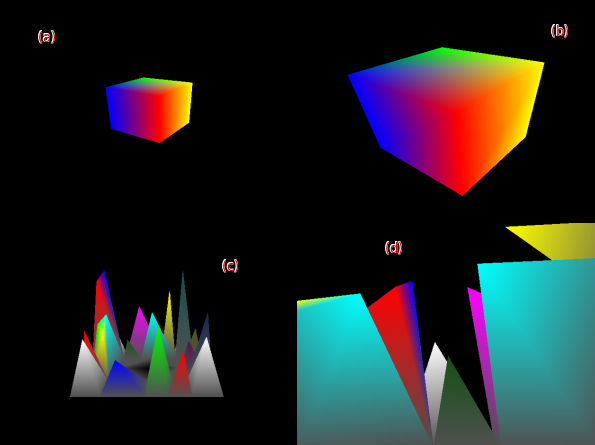
\includegraphics[scale=0.5]{images/rendered models.png}}
    \caption{Куб и горы. \\ На рисунках изображены куб и горы --- вдали и вблизи соответственно. }
    \label{rendered models}
\end{figure}

\begin{table}[ht]
	\begin{center}
	\begin{tabular}{|c|c|c|c|c|c|c|} \cline{2-7}
		\multicolumn{1}{c|}{} & \multicolumn{3}{|c|}{Куб} & \multicolumn{3}{|c|}{Горы} \\ \cline{2-7}
		\multicolumn{1}{c|}{} & Вдали & Вблизи & Min & Вдали & Вблизи & Min \\ \hline
		$640 \times 480$ & 70 & 60 & 21 & 60 & 38 & 13 \\ \hline
		$1280 \times 720$ & 28 & 21 & 11 & 25 & 14 & 7 \\ \hline
		$1920 \times 1080$ & 10 & 8 & 5 & 10 & 6 & 3 \\ \hline
	\end{tabular}
	\end{center}
	\caption{Результаты тестирования.}
	\label{testing results}
\end{table}

Как можно видеть, при маленьком разрешении разница FPS вдали практически не ощущается, а вблизи почти двукратная.
При среднем разрешении наблюдается похожий результат, а при максимальном разница практически отсутствует.
Во всех случаях при уменьшении расстояния количество FPS падает, так как увеличивается количество пикселей, которые покрывает итоговое изображение на экране монитора.
Причём клиппинг хоть и влияет достаточно сильно на производительность, в данных примерах его эффект не так силён.
В случае максимального разрешения мы получаем маленький FPS независимо от расстояния.
Это связано с тем, что всё время уходит на инициализацию структур для работы с большим количеством пикселей.
В данном случае эффект будет тем же, даже если запустить рендерер с пустой сценой.

\newpage

% Здесь автоматически генерируется библиография. Первая команда задает стиль оформления библиографии, а вторая указывает на имя файла с расширением bib, в котором находится информация об источниках.
\bibliographystyle{plainurl}
\bibliography{bibl}

% Здесь текст документа заканчивается
\end{document}
% Начиная с этого момента весь текст LaTeX игнорирует, можете вставлять любую абракадабру.
